\documentclass[aspectratio=169,11pt]{beamer}

\usetheme{Madrid}
\usecolortheme{seahorse}
\setbeamertemplate{navigation symbols}{}
\setbeamertemplate{footline}[frame number]

\usepackage[T1]{fontenc}
\usepackage[utf8]{inputenc}
\usepackage{amsmath}
\usepackage{tikz}
\usetikzlibrary{arrows.meta,positioning,shapes.geometric}

\title[BICEP Dust Simulations]{Dust Simulations for BICEP/Keck}
\subtitle{Where should we start, and how should we extrapolate?}
\author{}
\date{\today}

\newcommand{\bk}{BICEP/Keck}
\newcommand{\Planck}{\textit{Planck}}
\newcommand{\sed}{SED}
\newcommand{\st}{\mathrm{ST}}

\begin{document}

\begin{frame}
  \titlepage
\end{frame}

\begin{frame}{The goal}
  \begin{center}
    \Large
    Build realistic dust foreground simulations for the \bk{} field.

    \vspace{0.8cm}
    Use them to test whether foreground complexity can bias the recovered value of $r$.
  \end{center}
\end{frame}

\begin{frame}{What BICEP/Keck needs}
  \begin{columns}[T,onlytextwidth]
    \begin{column}{0.47\textwidth}
      \textbf{Maps}
      \begin{itemize}
        \item Independent realizations
        \item BICEP patch
        \item $N_{\rm side}=512$.
      \end{itemize}
    \end{column}

    \begin{column}{0.47\textwidth}
      \textbf{Checks}
      \begin{itemize}
        \item Right dust amplitude
        \item Useful over $30<\ell<500$
        \item Controlled frequency behavior
      \end{itemize}
    \end{column}
  \end{columns}

  \vspace{0.55cm}
  \begin{center}
    \Large
    Not a reconstruction of the real sky: an ensemble of plausible skies.
  \end{center}

  \vspace{0.35cm}
  \begin{center}
    \normalsize
    The range $30<\ell<500$ covers the degree scales used by \bk{}, especially
    the $r$-sensitive region around $\ell\simeq80$.
  \end{center}
\end{frame}

\begin{frame}{Our proposed route}
  \begin{center}
  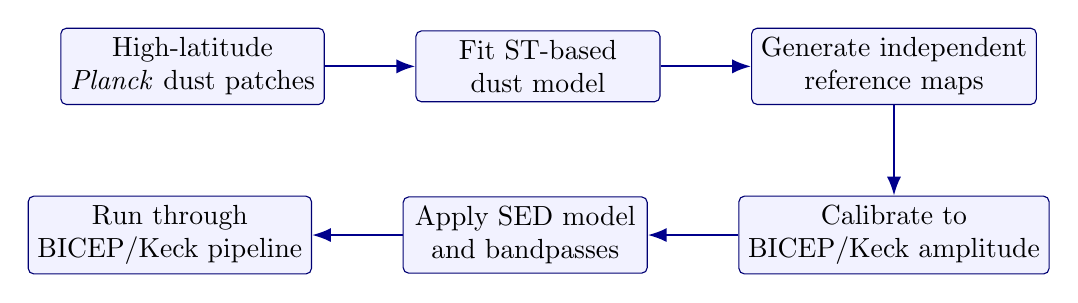
\begin{tikzpicture}[
      node distance=1.15cm,
      box/.style={rectangle, rounded corners=2pt, draw=blue!45!black, fill=blue!5, minimum width=3.1cm, minimum height=0.9cm, align=center},
      arrow/.style={-{Latex[length=2.4mm]}, thick, blue!55!black}
    ]
    \node[box] (data) {High-latitude\\\Planck{} dust patches};
    \node[box, right=of data] (stats) {Fit ST-based\\dust model};
    \node[box, right=of stats] (gen) {Generate independent\\reference maps};
    \node[box, below=of gen] (amp) {Calibrate to\\\bk{} amplitude};
    \node[box, left=of amp] (sed) {Apply SED model\\and bandpasses};
    \node[box, left=of sed] (test) {Run through\\\bk{} pipeline};

    \draw[arrow] (data) -- (stats);
    \draw[arrow] (stats) -- (gen);
    \draw[arrow] (gen) -- (amp);
    \draw[arrow] (amp) -- (sed);
    \draw[arrow] (sed) -- (test);
  \end{tikzpicture}
  \end{center}
\end{frame}

\begin{frame}{The central question}
  \begin{center}
    \Huge
    At what frequency do we build first?

    \vspace{1.0cm}
    \Huge
    How do we extrapolate?
  \end{center}
\end{frame}

\begin{frame}{Mathematical target}
  \small
  We want an ensemble of synthesized foreground maps
  \[
    \left\{\tilde{\mathbf s}_{\nu}^{\prime(a)}\right\}_{a=1}^{N_{\rm sim}},
    \qquad
    \tilde{\mathbf s}_{\nu}^{\prime(a)}
    =
    \left(\tilde I_\nu^{\prime(a)},\tilde Q_\nu^{\prime(a)},\tilde U_\nu^{\prime(a)}\right),
  \]
  on the \bk{} patch and at the \bk{} bandpasses.

  \vspace{0.35cm}
  In compact form, construct a distribution $\mathcal P_\Theta$ such that
  \[
    \mathbb E_{\mathcal P_\Theta}
    \left[
      \Phi(\tilde{\mathbf s}_{\nu_0}^{\prime},\tilde I^{\prime})
    \right]
    \simeq
    \widehat\Phi_{\rm HL},
  \]
  \[
    D_\ell^{BB,d}
    \simeq
    A_{d,\nu_0}^{\rm BK}
    \left(\frac{\ell}{80}\right)^{\alpha_d},
    \qquad
    30 \lesssim \ell \lesssim 500.
  \]
\end{frame}

\begin{frame}{Reference-frequency maps}
  \small
  Starting from high-latitude \Planck{} patches, synthesize maps at a reference frequency $\nu_0$:
  \[
    \tilde{\mathbf s}_{\nu_0}^{\prime(a)}
    =
    \operatorname*{arg\,min}_{\mathbf u}
    \left[
      \left\|
        \Phi_{\st}(\mathbf u,\tilde I_{\rm aux}^{\prime(a)})
        -
        \widehat\Phi_{\rm HL}
      \right\|_2^2
      +
      \lambda_{\rm PS}
      \left\|
        \widehat D_\ell^{BB}(\mathbf u)
        -
        D_{\ell,{\rm target}}^{BB,\nu_0}
      \right\|_2^2
    \right].
  \]

  \vspace{0.35cm}
  Then calibrate on the \bk{} mask:
  \[
    \tilde{\mathbf s}_{\nu_0}^{\prime(a)}
    \leftarrow
    \alpha_a\,\tilde{\mathbf s}_{\nu_0}^{\prime(a)},
    \qquad
    \alpha_a =
    \left(
      \frac{A_{d,\nu_0}^{\rm BK}}
           {\widehat A_{d,\nu_0}^{(a)}}
    \right)^{1/2}.
  \]
\end{frame}

\begin{frame}{SED model: three cases}
  \small
  Starting from reference-frequency maps, we need a model for
  $\tilde Q_\nu'(\hat n),\tilde U_\nu'(\hat n)$ at the \bk{} bandpasses.

  \vspace{0.25cm}
  \begin{enumerate}
    \item \textbf{Spatially varying SED}
    \[
      \beta_d(\hat n),\,T_d(\hat n)
    \]

    \item \textbf{Multi-layer dust}
    \[
      \tilde Q_\nu'(\hat n)
      =
      \sum_{k=1}^{K}
      \tilde Q_{k,\nu_0}'(\hat n)\,
      f_d(\nu;\beta_{d,k}(\hat n),T_{d,k}(\hat n)).
    \]
    Here $k$ labels distinct dust layers or components along the line of sight.

    \item \textbf{Stochastic SED fluctuations}\\
    small-scale SED variations tuned to a target decorrelation level.
  \end{enumerate}
\end{frame}

\begin{frame}{Decorrelation diagnostic}
  \small
  For two frequencies, measure on the \bk{} mask:
  \[
    \Delta_d(\nu_1,\nu_2;\ell)
    =
    \frac{C_\ell^{BB,d}(\nu_1\times\nu_2)}
    {\sqrt{C_\ell^{BB,d}(\nu_1\times\nu_1)
           C_\ell^{BB,d}(\nu_2\times\nu_2)}}.
  \]

  \vspace{0.5cm}
  \begin{center}
    \Large
    Compare $\Delta_d$ with the \bk{} decorrelation constraint.
  \end{center}

  \vspace{0.25cm}
  \begin{center}
    BK18 peaks at no detected decorrelation; strongly decorrelated models
    should be treated as labelled stress tests.
  \end{center}
\end{frame}

\begin{frame}{End-to-end test}
  \begin{center}
    \Large
    Choose an input $r$ and generate a CMB realization.

    \vspace{0.45cm}
    Add $n$ and one dust realization:
    \[
      {\rm CMB}(r_{\rm input}) + n^{(a)}
      + \tilde{\mathbf s}_{\nu}^{\prime(a)}.
    \]

    \vspace{0.45cm}
    Run the \bk{} likelihood and measure how dust changes the recovered value:

    \[
      \Delta r
      =
      \widehat r_{\rm recovered}
      -
      r_{\rm input}.
    \]
  \end{center}
\end{frame}

\section{Current implementation}

\begin{frame}{Current ST synthesis script}
  \small
  The script \texttt{hlst.py} is our current debugging path for the
  reference-frequency dust synthesis.

  \vspace{0.35cm}
  \begin{itemize}
    \item Start from component-separated \Planck{} patch products:
    \[
      (Q_i,U_i), \qquad i\in\mathcal I_{\rm HL}.
    \]

    \item Compute ST targets separately for $Q$ and $U$:
    \[
      \widehat\Phi_Q =
      \frac{1}{|\mathcal I_{\rm HL}|}
      \sum_{i\in\mathcal I_{\rm HL}}\Phi_{\st}(w_i^Q Q_i),
      \qquad
      \widehat\Phi_U =
      \frac{1}{|\mathcal I_{\rm HL}|}
      \sum_{i\in\mathcal I_{\rm HL}}\Phi_{\st}(w_i^U U_i).
    \]

    \[
      w_i^Q=\frac{\sigma_Q(178)}{\sigma_Q(i)},
      \qquad
      w_i^U=\frac{\sigma_U(178)}{\sigma_U(i)}.
    \]
    For debugging we can set $w_i^Q=w_i^U=1$.

    \item Synthesize one $Q$ map and one $U$ map matching these average targets.
  \end{itemize}
\end{frame}

\begin{frame}{What is fixed, what is adjustable}
  \small
  \begin{columns}[T,onlytextwidth]
    \begin{column}{0.47\textwidth}
      \textbf{Fixed for the target}
      \begin{itemize}
        \item Target patch STs use non-periodic boundaries.
        \item ST coefficients are normalized.
        \item $Q$ and $U$ are treated independently.
      \end{itemize}
    \end{column}

    \begin{column}{0.47\textwidth}
      \textbf{Debug knobs}
      \begin{itemize}
        \item Patch list, currently patch 129.
        \item Optional map-amplitude normalization to patch 178.
        \item Periodic or non-periodic synthesis.
      \end{itemize}
    \end{column}
  \end{columns}

  \vspace{0.45cm}
  The output is a compact diagnostic: synthesized $Q$, $U$, $P$, and the
  two loss curves.
\end{frame}

\begin{frame}{Your contribution}
  \begin{center}
    \Large
    Choose a physically sensible extrapolation strategy.

    \vspace{0.8cm}
    Identify the minimal SED complexity we need.

    \vspace{0.8cm}
    Help define what ``compatible with dust data'' means.
  \end{center}
\end{frame}

\begin{frame}{Decisions to leave with}
  \begin{itemize}
    \item Reference frequency for the first maps.
    \item SED prescription for the first extrapolation.
    \item How to allow or limit decorrelation.
    \item Diagnostics to send with the maps.
  \end{itemize}
\end{frame}

\end{document}
